\documentclass[a4paper,11pt]{article}
\usepackage[utf8]{inputenc}
\usepackage[paper=a4paper, hmargin=1.5cm, bottom=1.5cm, top=3.5cm]{geometry}
\usepackage[T1]{fontenc}
\usepackage[spanish]{babel}
\usepackage[colorlinks=true, linkcolor=blue]{hyperref} %Links para el indice.
\usepackage{amsfonts}
\usepackage{verbatim}
\usepackage{listings}
\usepackage{caption}
\usepackage{subcaption}

\usepackage[section]{placeins}
\usepackage{float}
%\usepackage{adjustbox}
\usepackage{amsmath}
\usepackage{blindtext}
\usepackage{sidecap}
\usepackage{color}
\usepackage{graphicx}

% \newcommand{\real}{\hbox{\bf R}}

\title{Trabajo Práctico de Ingeniería de Software I}

\begin{document}

\maketitle

\begin{center}
	Universidad de Buenos Aires - Departamento de Computaci\'on - FCEN
\end{center}

\vspace{2cm}
Integrantes:

\begin{itemize}
	\item Castro, Dami\'an L.U.: 326/11  \verb+ltdicai@gmail.com+
	\item Matayoshi, Leandro L.U.: 79/11 \verb+leandro.matayoshi@gmail.com+
	\item Melnik, Jonathan L.U.: 571/09 \verb+jonathanmelnik@gmail.com+
	\item Santos, Martín L.U.: 413/11 \verb+martin.n.santos@gmail.com+
	\item Szyrej, Alexander L.U.: 642/11   \verb+alexanderszyrej@gmail.com+
	
\end{itemize}

\newpage

\tableofcontents

\newpage

\section{Introducción}
Nuestro prestigioso equipo de desarrolladores de software llamado ''Grupo 4'' ha sido solicitado por el gobierno de
Mar Chiquita para el desarrollo de un sistema que administre su nueva red de ciclovías, con el objetivo de acercar
a los habitantes a este nuevo medio de transporte y lograr estimular su uso.

Los empleados del gobierno nos han compartido sus expectativas en que las ciclovías contribuyan a aliviar la 
red de transporte público y disminuir la cantidad de automóviles particulares en circulación. Al mismo tiempo
creen que el uso de las bicicletas es una buena manera intentar reducir el sobrepeso que sufre la mayor parte 
de la población, al atacar una de las principales causas como lo es el sedentarismo. 

Al mismo tiempo, algunos futuros usuarios nos han hecho llegar sus comentarios e inquietudes respecto al uso que
desean darle a la red: Disponibilidad en las estaciones del centro durante las horas pico, preocupación respecto
a la caída de conexión de internet en alguna de las estaciones, reposición de bicicletas cuando se agota el stock,
buena disponibilidad de las mismas, protección e integridad de los datos de los usuarios, entre otros. 
Los empleados del gobierno que supervisarán el sistema también quieren contar con información relevante (estadísticas,
comentarios de los usuarios, etc) que les permitan tomar mejores decisiones a futuro.

Considerando todos estos puntos, planificamos y diseñamos una serie de documentos a través de los cuales pretendemos 
llegar a un acuerdo con los stakeholders respecto a los requerimientos que debe cumplir nuestro sistema.

Para ello, debemos asegurarnos
de haber comprendido correctamente los objetivos que se esperan de este software, y aquellos que han motivado la
creación del mismo. La creación de un diagrama de objetivos nos pareció una buena herramienta para establecer
una base concreta sobre la cual trabajar.

Al mismo tiempo debemos ponernos de acuerdo respecto al alcance de nuestro software.
Una buena aproximación es, en primer lugar, determinar el conjunto de todos los eventos que se relacionan con 
la red de ciclovías y el sistema administrador a desarrollar, distinguiendo entre aquellos que se corresponden 
exclusivamente con la red, aquellos que lo hacen exclusivamente con el sistema a desarrollar y finalmente, aquellos 
eventos que relacionan ambas componentes. Para ello decidimos utilizar el modelo de Jackson.
Luego, utilizando los eventos relevantes, diseñar un diagrama de contexto mostrando
las interacciones entre los distintos agentes, y entre estos y el sistema a desarrollar.
\subsection{Propuesta a los stakeholders}

El gobierno de Mar Chiquita atraviesa un colapso general del transporte público y al mismo tiempo, un incremento reciente en la cantidad de automóviles particulares en circulación. También se ha puesto en evidencia el problema de salud general que atraviesa de Mar Chiquita, ya que estadísticas recientes muestran un alto índice de obesidad y sedentarismo de la gente de la localidad.

Se nos ha comunicado que una estrategia a seguir para aliviar estas problemáticas es estimular el uso de la nueva Red de Ciclovías de Mar Chiquita.

Modificar la cotidianeidad de las personas es un objetivo difícil de lograr, pero confiamos en que la realización de un plan de acción completo y de alcance general que concientize a la población, mejore la infraestructura y que facilite el uso de la Red podrá lograr dicho objetivo.

Con ese objetivo en mente, “Grupo 4”, elaboró una propuesta para llevar a cabo la estrategia planteada.

El relevamiento de los requerimientos y objetivos, ha puesto en evidencia la necesidad de proporcionar un sistema informático que permita resolver la disponibilidad de bicicletas, principalmente en las horas pico, facilitar el retiro de las bicicletas, permitir a los usuarios acceder a servicios de la Red mediante Internet para el registro y chequeo del estado de la red y disponibilidad de las bicicletas en las estaciones de la Red y que la administración a su vez pueda ser realizada mediante un sistema centralizado a través de Internet. 

Nuestra propuesta consta de distintas mecánicas que, instrumentadas en conjunto, favorecerán la adopción de la Red a la vida cotidiana de las personas y lograrán que la población de Mar Chiquita acceda a un sistema de Red de Ciclovías gratuito, confiable, efectivo y de nivel internacional.


\newpage

\section{Eventos del modelo de Jackson}

Con la intención de concretizar los requerimientos de la propuesta utilizamos el ampliamente conocido modelo de Jackson: 
\footnote{\url{http://users.mct.open.ac.uk/mj665/icse17kn.pdf}}

Se basa en estudiar los requerimientos, separando los fenómenos que pertenecen al Mundo(World), la Interfaz y el Sistema(Machine). Esta distinción permite exhibir el propósito del sistema, el cual se encuentra en el Mundo y delimitar el alcance
del mismo. 

Hicimos un relevamiento, y a continuación exponemos un listado con todos los fenómenos(eventos o situaciones observables) que encontramos.
Los fenómenos pertenecientes al Mundo serán objetivos relevados y las presunciones que elaboramos y los que pertenecen a la Interfaz son los requerimientos del sistema que responden a los eventos en el Mundo.


\vspace{1cm}
\textbf{\underline{W: World}}

\begin{itemize}
\item Usuario va a buscar una bicicleta a una estación de la periferia.
\item Usuario va a buscar una bicicleta a una estación del centro.
\item Usuario retira una bicicleta de alguna estación
\item Usuario devuelve una bicicleta en alguna estación
\item Usuario se identifica en una estación, presentando DNI.
\item Usuario se desplaza entre estación y estación.
\item Los camiones de la empresa de transporte proveen una estación con más bicicletas.
\item Los camiones de la empresa de transporte retiran bicicletas de una estación.
\item Un empleado de gobierno provee a la empresa de transporte de mayor cantidad de bicicletas.
\item Empleado de estación rechaza solicitud de retiro de bicicleta debido a penalización.
\item Una estación no dispone de bicicletas para retirar
\item Empleado de gobierno inaugura estación añadiéndola a la red de ciclovías.
\item Empleado de gobierno contrata persona para que trabaje como empleado de estación.
\item Usuario nunca devuelve una bicicleta
\item Usuario (que ya dispone de una) solicita otra bicicleta.
\item Alguien se hace pasar por un usuario para retirar/devolver una bicicleta
\item La gente se traslada ida y vuelta a su trabajo/casa en una franja horaria reducida, llamada ''hora pico''
\item Usuario sufre un accidente.
\item La bicicleta sufre un desperfecto.
\item Usuario rompe una bicicleta
\item Usuario no cumple con las normativas para el uso de la red de ciclovías.
\item Usuario olvida contraseña
\item Usuario espera por bicicleta
\item Usuario devuelve una bicicleta que no está en condiciones.
\item Usuario devuelve una bicicleta fuera de horario.
\item Usuario devuelve una bicicleta en una estación cerrada
\item Ninguna estación dispone de bicicletas
\item Un nuevo usuario no provee la información necesaria para inscribirse.
\item Empleado le entrega una bicicleta a un usuario que no está registrado.
\item Empleado le entrega una bicicleta a un usuario que está penalizado.
\item Gobierno entrega más bicicletas a la empresa de transportes.
\item Sistema pierde la conexión.
\item La empresa de transporte no cumple con el tiempo estimado en trasladar las bicicletas.
\item Una estación queda aislada
\item La empresa de transporte no se puede movilizar.
\item Muchos usuarios se registran a la vez.
\end{itemize}

\vspace{1cm}
\textbf{\underline{I: Interface}}

\begin{itemize}

\item Empleado de estación envía (via internet) información de autenticación de un usuario para ser validada por el sistema.
\item Empleado de estación ingresa (via internet) en el sistema modificación de stock de bicicletas.
\item Empleado de estación ingresa (via internet) en el sistema penalización a usuario.
\item Empleado de estación ingresa (via internet) información de bicicleta en mal estado.
\item Empleado de estación envía información de autenticación de un usuario para ser validada por el sistema via SMS, debido
a la pérdida de conexión de internet de la estación en donde trabaja.
\item Empleado de estación ingresa en el sistema modificación de stock de bicicletas via SMS, debido
a la pérdida de conexión de internet de la estación en donde trabaja.
\item Empleado de estación ingresa en el sistema penalización a usuario via SMS, debido
a la pérdida de conexión de internet de la estación en donde trabaja.
\item Empleado de estación ingresa información de bicicleta en mal estado via SMS, debido
a la pérdida de conexión de internet de la estación en donde trabaja.
\item Empleado de estación consulta datos de usuario: si existe alquiler actual, si el usuario está penalizado
actualmente.


\item Empleado de gobierno realiza cualquiera de las acciones que puede realizar el empleado de estación (vía internet
o SMS). Por ejemlo, empleado de gobierno ingresa modificación de stock.
\item Empleado de gobierno realiza consulta de estadísticas relevantes al sistema.
\item Empleado de gobierno realiza consulta sugerencias de usuarios al sistema.
\item Empleado de gobierno ingresa nueva estación al sistema.
\item Empleado de gobierno ingresa nuevo empleado en el sistema.
\item Empleado de gobierno da de baja empleado en el sistema.
\item Empleado de gobierno actualiza estado de la empresa de transporte

\item Sistema solicita a movilización de bicicletas a la empresa de transporte.
\item Sistema devuelve al empleado de estación el resultado de autenticación válida o inválida
\item Sistema envía a usuario información de stock de bicicletas disponibles para una determinada estación.
\item Sistema envía a usuario tiempo restante para que haya una bicicleta disponible en una determinada estación, en el caso
de que no haya stock.
\item Sistema envía a usuario información acerca de sus penalizaciones.

\item Usuario se registra en el sistema.
\item Usuario se loguea en el sistema.
\item Usuario ingresa sugerencia en el sistema.
\item Usuario completa encuesta respecto a un nuevo lugar en donde agregar una nueva estación.
\item Usuario ingresa comentarios respecto al cambio en su estado de salud desde que es usuario de la red.
\item Usuario consulta stock de bicicletas en una determinada estación.
\item Usuario consulta acerca de sus penalizaciones.

\end{itemize}


\vspace{1cm}
\textbf{\underline{M: Machine}}

\begin{itemize}
\item El sistema calcula el mejor conjunto de estaciones que disponen de bicicletas para otra estación.
\item El sistema detecta que una estación se ha quedado sin bicicletas.
\item El sistema detecta que en una estación sobran bicicletas, al contrastar la cantidad actual con los datos
de las estadísticas recientes.
\item El sistema actualiza el estado de un usuario.
\item El sistema detecta una discrepancia entre la solicitud de un usuario y el estado del usuario en el sistema.
\item El sistema registra estadísticas relevantes
\item El sistema actualiza el estado de una estación.
\item El sistema recalcula distribución de bicicletas cuando se agrega una estación a la red.
\end{itemize}




\newpage
\section{Diagrama de contexto}
Es de nuestro interés exhibir cómo es la interacción entre los distintas entidades del mundo y el sistema que diseñamos.

A continuación presentamos un diagrama de Contexto. Este tipo de diagrama separa los fenómenos de las entidades que los controlan y/o monitorean. Cada una de estas entidades o agentes, cumple un rol determinado e interactúa con otros agentes y/o con el sistema. Además, nos permite mostrar de forma concreta el alcance de nuestro software.

El  diagrama fue armado en base a las siguientes decisiones en las ramas que constituían o-refinamientos en su diagrama de objetivos correspondiente:

\begin{itemize}
\item Las personas se registran como usuarios de la red de ciclovías vía internet (registración automatizada).
\item La asistencia personalizada para la registración es efectuada en las estaciones por los empleados que allí trabajan.
\item Durante las horas pico, la demanda es satisfecha agregando mayor cantidad de empleados en las estaciones.
\item Los usuarios se registran brindando DNI, mail, teléfono de contacto, domicilio y contraseña para poder loguearse, 
\end{itemize}

Como en este tipo de diagrama no existe el concepto de herencia entre actores, agregamos (*1) para expresar que el
empleado de gobierno también controla y monitorea los mismos fenómenos que un empleado de estación. A saber:
Ingresar bicicleta en mal estado, validar autenticación, modificar stock, ingresar penalizaciones, registrar usuarios y consultar datos de usuario.

(*2) Los usuarios pueden dejar comentarios tanto respecto a salud, funcionamiento general del sistema y lugares donde agregar nuevas estaciones.
También pueden completar las encuestas en relación a este último punto.

\begin{figure}[H]
	\begin{center}
		  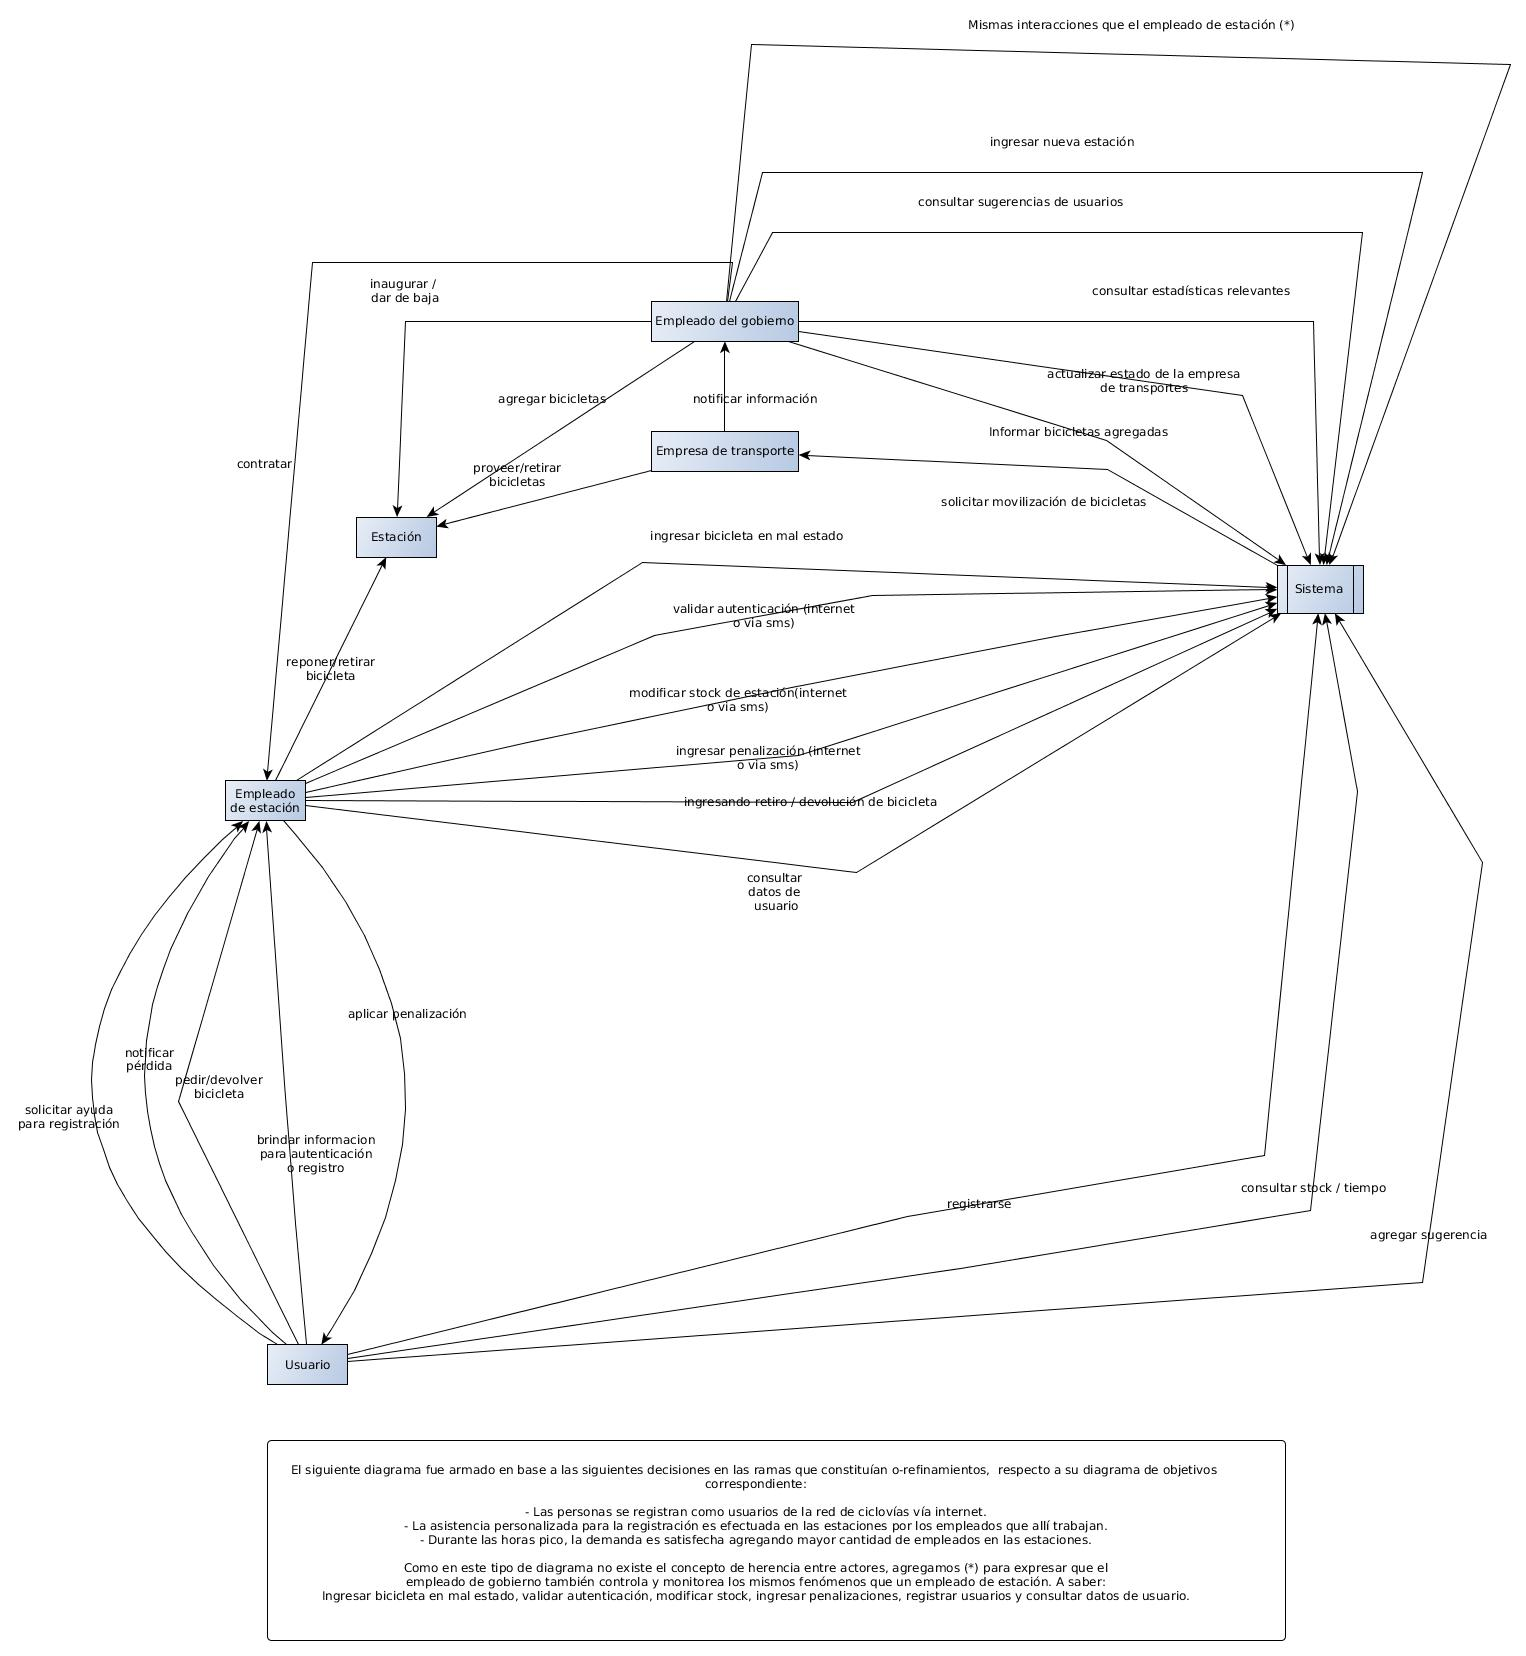
\includegraphics[scale=0.35]{diagrama_contexto.jpg}
		  \caption{Diagrama de contexto}
		  \label{fig:contra1}
	\end{center}
\end{figure}

Los usuarios comienzan registrándose por internet brindando los datos requeridos. Entre ellos se destacan principalmente el número de DNI y el nombre completo, ya que ambos serán utilizados
para validar la identidad cada vez que quieran hacer uso de la red. 

En el caso de tener dificultades para completar este proceso pueden acercarse a una de las estaciones y solicitar ayuda a uno de los empleados.
Siempre que un usuario quiera acercarse a una estacion para retirar una bicicleta tiene la opción de consultar previamente la disponibilidad de stock. En caso de estar agotado, el sistema informará el tiempo
estimado en el cual se repondrá.

A la hora de alquilar una bicicleta el usuario le comunica su nombre completo y su DNI al empleado. El empleado de estación valida con el sistema la información recibida y posteriormente le comunica
los resultados. Si existe un problema de autenticación el empleado le solicita que se registre nuevamente. De lo contrario el usuario será autenticado con éxito. Posteriormente, el empleado chequea 
su estado, en donde busca existencia de alquileres pendientes o penalizaciones que no han sido cumplidas. En el caso de no encontrar anormalidades, el usuario
recibe una bicicleta para ser utilizada, la cual deberá devolver en un lapso de tiempo menor a 1 hora.

Si el usuario pierde la bicicleta, o la misma sufre un desperfecto importante durante su uso debe notificarlo en alguna de las estaciones. Ambos hechos serán sancionados e ingresados al sistema
por parte del empleado. Por el contrario, si el usuario devuelve la bicicleta en tiempo y forma, el alquiler finaliza y el usuario podrá retirar nuevamente otra bicicleta sin ningún inconveniente.

Los usuarios pueden dejar sugerencias y comentarios en el sistema, que serán tenidas en cuenta por los empleados del gobierno de Mar Chiquita.

El empleado de estación es el encargado de validar la autenticación de los usuarios, otorgar y recibir las bicicletas, consultar el estado de los usuarios, aplicar las penalizaciones (negando la posibilidad
de que efectúen alquileres), colaborar con la empresa de transportes en la movilización (cargando y descargando las
bicicis) e ingresar los datos al sistema. Entre los datos que puede registrar se destacan: la modificación del stock de bicis, el inicio o cierre de un alquiler, 
el ingreso de una penalización, el ingreso de una bicicleta en mal estado o de un extravío.

El stock en una estación se modifica cuando se retiran bicicletas para satisfacer un pedido, o cuando se reciben bicicletas debido a un pedido. En ambos casos, es el empleado de estación quien actualiza esta información en el sistema.

El stock disponible en cada estación a cada hora, y las movilizaciones entre estaciones son manejadas en su totalidad por parte del sistema mediante un algoritmo
, ya que este último es el que dispone de toda la información necesaria para calcular la mejor distribución (considerando que la demanda es mayor en las estaciones del centro en el horario pico). 
Los empleados no pueden realizar pedidos a la empresa de transporte ya que es responsabilidad del sistema, aún cuando la estación agota su stock.

El sistema provee una api que permite cargar y enviar los datos a través de sms's enviados por los empleados en los casos en los que se pierde la conexión a internet en sus respectivas estaciones. 

Las bicicletas están distribuídas en las estaciones. Periódicamente nuevas bicicletas son agregadas por parte de los funcionarios del gobierno para reponer las que se han roto o han sido extraviadas.
Simultáneamente las nuevas bicicletas son ingresadas al sistema, pasando a formar parte de la red.

La empresa de transporte responde a los pedidos que recibe por parte del sistema. En el caso de que surja un inconveniente (por ejemplo, menor disponibilidad de camiones para traslados o imposibilidad de realizar
determinados pedidos), la misma le informa a uno de los empleados del gobierno y este último carga dicha información en el sistema. 
 
El sistema calcula y actualiza constantemente estadísticas recolectadas a partir de los alquileres, las penalizaciones, el stock en cada momento del día, etc. Dicha información es utilizada para mejorar
el algoritmo de predicción y distribución, y al mismo tiempo puede ser consultada por los empleados del gobierno.

Estos últimos pueden realizar cualquier actividad asociada a un empleado de estación (no así a la inversa). (Consultar datos de usuarios, cargar y cerrar alquileres, etc.). A su vez, son responsables
de contratar y dar de baja a empleados (tanto de gobierno como de estaciones), inaugurar y dar de baja estaciones, consultar las sugerencias y validar los registros. 
Este último punto es de fundamental importancia, ya que los usuarios no pueden comenzar a retirar bicicletas si sus registros no han sido validados. 

\section{Escenarios informales}

\subsection{Algunos escenarios posibles}
\begin{itemize}

\item Un señor cansado de sufrir el tránsito vehicular de Mar Chiquita observa un anuncio en donde se informan los beneficios de usar la nueva red de ciclovías que ofrece el Gobierno. Decide darle una oportunidad. Ingresa al sitio web que vio en el anuncio y comienza a llenar el formulario de inscripción para utilizar el servicio. 

Una vez registrado, el individuo se acerca a la estación más cercana a su hogar. Se encuentra con un empleado que le solicita el DNI. El usuario se lo da y el empleado realiza ciertos chequeos en la computadora de la estación. Verifica que se encuentra todo en orden y procede a darle una bicicleta. El usuario la utiliza y la devuelve en otra estación pasado el tiempo reglamentario. El empleado le notifica que cometió una infracción y le aplica una penalización que le prohibe utilizar bicicletas por una semana. El usuario se retira de la estación. Luego de 3 días el usuario vuelve a acercarse a una estación para retirar una bicicleta. Para ello le entrega su DNI al empleado. Este le informa que se encuentra penalizado y que debe esperar 4 días más para retirar una bicicleta. El usuario se retira.

\item Juan es empleado de una estación del centro de la red de ciclovías. Comienza su jornada laboral. Durante el transcurso del día se acercan varios usuarios con la intención de utlizar bicicletas para lo cual Juan debe realizar registros y autenticaciones de los mismos. Pasan las horas y Juan observa que las bicicletas comienzan a escasear. Luego de unos minutos arriba un camión lleno de bicicletas. Juan actualiza el stock de bicicletas presentes en la estación.
Llega la hora pico y Juan observa que llegan nuevos empleados a la estación. Al rato el caudal de usuarios que se aproxima comienza a aumentar. Aún así el tiempo de espera sigue siendo reducido. En cierto momento se pierde la conexión a internet y Juan comienza a utlizar el servicio de mensajeria de su celular para que el servicio pueda seguir funcionando. Termina la jornada laboral.

\end{itemize}

\begin{itemize}
\item Luciano, un empleado de gobierno, está interesado en conocer la opinión general de los usuarios que han utilizado la
red de ciclovías durante el último mes. Para ello consulta en primer lugar el tiempo promedio que han tenido que esperar   
los usuarios por las bicicletas durante las horas pico en las estaciones del centro. Esto es muy importante, ya que 
demasiada espera hace que los usuarios no estén satisfechos.

Luego de analizar estas estadísticas (y otras más que provee el sistema) procede a leer las sugerencias y quejas ingresadas
por los usuarios. Es en este momento cuando descubre que una cantidad significante de usuarios coincide en que sería muy
beneficioso añadir una nueva estación entre ''Mar azulado'' y ''Descanso veraniego'' (otras 2 estaciones céntricas 
existentes). Los usuarios alegan que este tramo es demasiado extenso y que deben realizar gran parte del recorrido a pie
cuando las oficinas en donde trabajan quedan entre ambas estaciones.

Considerando estos hechos, Luciano redacta un informe y lo presenta ante el Ministerio de transporte de Mar Chiquita, cuya
junta autoriza (luego de un riguroso análisis) la creación de la nueva estación.

Dos meses después, luego de realizar las obras de infraestructura correspondiente, Luciano junto a otros miembros del
ministerio inauguran orgullosos la nueva estación y la ingresan al sistema, para que pase a formar parte de la red de ciclovías.

\end{itemize}

\end{document}
